
%(BEGIN_QUESTION)
% Copyright 2009, Tony R. Kuphaldt, released under the Creative Commons Attribution License (v 1.0)
% This means you may do almost anything with this work of mine, so long as you give me proper credit

Here is an oscilloscope's view of an seven-bit data stream sent asynchronously with no parity bit, using {\it NRZ} (Non-Return to Zero) encoding:

$$
\includegraphics[width=15.5cm]{i02366x01.eps}$$

Identify the binary data represented by this waveform.

\underbar{file i02366}
%(END_QUESTION)





%(BEGIN_ANSWER)

$$\includegraphics[width=15.5cm]{i02366x02.eps}$$

%(END_ANSWER)





%(BEGIN_NOTES)

The trick to decoding data here is knowing there are {\it seven} data bits, and figuring out how wide each one is.

%INDEX% Networking, serial data: asynchronous data format
%INDEX% Networking, serial data: start bit
%INDEX% Networking, serial data: stop bit

%(END_NOTES)


